% Contribution chapter no. 3 (TOP20 pick 3, id Z-UO-TIERED) -- English translation of chapters/c03.tex
% Sources: papers/universal_optimality_tiered/ (universal_optimality_tiered.tex, gen_numbers.tex,
% publication_meta_v2.json), results/discovery/ledger/manuscript_audit_2026-10-11.md,
% papers/ar_yukawa_crystal/data/NUMERICS.md (erratum), TOP20.json.
\chapter[The triangle, the cheapest arrangement]{The triangle, the cheapest arrangement: verified consequences and a simulation}
\reference{Published on 11 October 2026.\\ v1: doi:10.5281/\\zenodo.23293112\\ v2: doi:10.5281/\\zenodo.23293429}

\section*{The idea in one picture}

\begin{analogie}
Lay identical marbles flat on a large tray, in a single layer, and imagine that they all push each other away a
little, even from afar. A theorem says which arrangement costs the least energy: the pattern of triangles, where each
marble has six neighbours, like the centres of the cells of a honeycomb. A simulation shakes the tray to see whether
the marbles find this pattern on their own.

\emph{Where the picture stops:} real marbles push only on contact, on a tray of finite size; the theorem speaks of a
repulsion acting at a distance, on an infinite plane, at a fixed density.
\end{analogie}

\section*{What was done}

In September 2026, OpenAI published a proof, produced by an AI and checked by computer, of a statement that the
literature described as an important open problem: for a wide family of repulsions, the triangular arrangement has the
smallest energy among all the ways of placing points in the plane at a given density. This chapter and the following
ones call this result ``the upstream theorem''. The work presented here draws consequences from it that are verified
by the machine, and confronts one physical case with a simulation.

Two consequences are proved. First, the triangular lattice, suitably stretched, is optimal at \emph{all} densities,
in the sense of a classical definition of ``universal optimality'' (in a slightly weaker version, which compares
averages in the sense of a lower limit). Second, the optimum is not unique: if one point is removed from the lattice,
neither the density nor the energy changes, and yet this lattice with a hole is not a displaced copy of the full
lattice.

\begin{encadre}
\textbf{To do with a pencil: why the lattice with a hole is not a copy.} A rigid motion (translation, rotation,
reflection) preserves midpoints: if $M$ is the midpoint of $P$ and $Q$, its image is the midpoint of the images. Write
$a\approx1.075$ for the spacing between neighbours. In the lattice with a hole, the points $(a,0)$ and $(2a,0)$
exist, and the point ``mirror image of $(2a,0)$ through $(a,0)$'' is $2(a,0)-(2a,0)=(0,0)$: that is the hole
(figure~\ref{fig:c03}a). If a motion sent the full lattice onto the lattice with a hole, two points $u$ and $v$ of the
full lattice would land on $(a,0)$ and $(2a,0)$. The point $2u-v$ is still in the full lattice, and it would land on
$(0,0)$, which is missing. Contradiction.

\textbf{The hole costs nothing on average.} In a disc of 1,000 points, removing one changes the average per point by a
factor of $1000/999\approx1.001$; with a million points, $1.000001$. In the limit, nothing at all.
\end{encadre}

On the physics side, the work studies the ``screened'' repulsion (called Yukawa), that of charged grains in a dusty
plasma: it weakens faster than ordinary electric repulsion, with a screening parameter $\kappa$. That it belongs to the
family of the theorem is, here, an argument written by AI agents, not checked by the machine \niveau{C} (it will be,
in Chapter~\ref{ch:c04}). A simulation of 288 particles, run with the CVODE solver rewritten in Rust by the project, lets each
disordered configuration slide down to an energy minimum. None of the 100 relaxations at $\kappa=2$, nor of the 50
at $\kappa=1$, went below the energy of the triangular lattice. Simulated annealing (heating, then cooling slowly)
found the perfect lattice only once in 20 in each family of starting points at $\kappa=2$, and failed the announced
criterion at $\kappa=1$.

\begin{figure}[htbp]
\centering
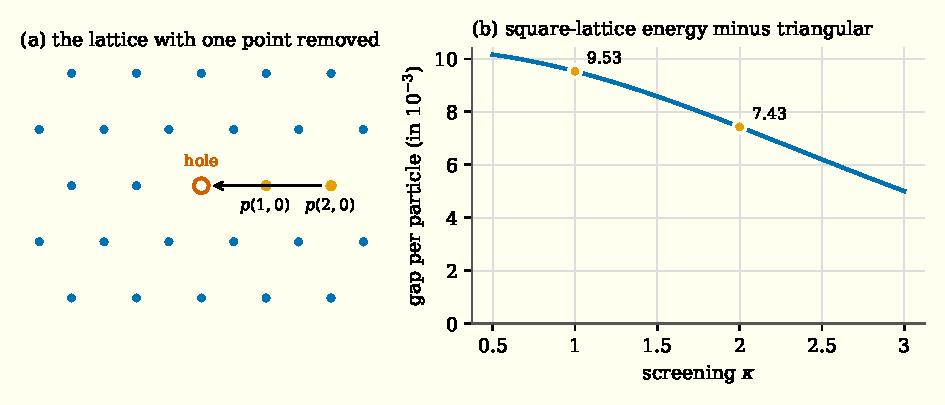
\includegraphics[width=\linewidth]{figures/c03_lacune}
\caption{(a) The argument of the hole. (b) Energy gap per particle, square lattice minus triangular lattice,
recomputed with the exact law, without cut-off (level X); at the marked points it gives back the exact values of
Chapter~\ref{ch:c04}, from which the values published on 11 October, with a cut-off, differ by at most $2.2\times10^{-6}$.}
\label{fig:c03}
\end{figure}

\section*{How we made sure it is not wrong}

\niveau{A} \emph{The judge looked.} The two consequences are Lean theorems (Lean is a program that checks every
logical step of a proof). They use only the three basic assumptions accepted everywhere, two deliberate traps (a proof
left blank, an invented axiom) were detected, and the module was replayed without error by a second checking program
on 26 October 2026. The simulation remains \niveau{X}: it guides, it proves nothing.

Every claim is filed in a register of 22 lines with its level of confidence. This register refuses to give the green
light: 6 lines of level A are still waiting for a person to check that the statement says what we think it says. The
author chose to publish with these flags visible and wrote this in the paper. An independent audit by another AI agent
asked for three text corrections, which were made, and a second review followed. This result, like the whole book,
was produced and audited by AI agents; no human specialist has reviewed it, and the upstream theorem itself has not
yet been evaluated by peers. In the simulation, the control cases behaved as expected: a perfect lattice stays in
place, a square lattice turns out to be unstable (72 directions in which the energy goes down), and a box that cannot
hold perfect triangles keeps its defects.

\section*{What this does not say}

\begin{limite}
\begin{itemize}
\item Everything rests on the upstream theorem, produced by an AI and not yet reviewed by peers.
\item The simulation cut the force off beyond a distance of 8. This cut-off lowered the energy by about $0.018$ at
$\kappa=1$, more than the square--triangle gap (about $0.0095$): an erratum, corrected in Chapter~\ref{ch:c04}.
\item The failure of annealing at $\kappa=1$ shows a weakness of the tool, not a flaw in the theorem.
\item Uniqueness among periodic arrangements is neither claimed nor studied.
\end{itemize}
\end{limite}

\section*{Going further}

This work serves as a template for everything that follows: the AI proposes, the computation explores, Lean judges,
the human decides whether to publish. Version 2 adds figures and laboratory protocols. Paper:
doi:10.5281/zenodo.23293429.
